\newcommand{\bmhMiscVersion}{v0.8-beta}

% --- language dependent typography stuff

\renewcommand{\fsNormal}{\fontsize{10pt}{14pt plus 0.1pt minus 0.1pt}}
\newcommand{\fsNormalB}{\fontsize{9.75pt}{13pt plus 0.1pt minus 0.1pt}}

\renewcommand{\fsSmall}{\fontsize{9pt}{11pt}}
\renewcommand{\fsSmall}{\fontsize{9pt}{11pt}}

\renewcommand{\say}[1]{„\textit{#1}“}
\setdefaultlanguage[spelling=new]{german}

% --- pdf metadata

\hypersetup{
	pdftitle={Battlemap Heroes},
	pdfsubject={Helden zum Quadrat!},
	pdfkeywords={Brettspiel, Rollenspiel, RPG, Regeln},
	pdfpagelayout=TwoPageRight,
}

% --- language macros --------------------------------------------------

\newcommand{\zB}{z.\,B.}

% ======================================================================
% texts
% ======================================================================

\newcommand{\bmh}{\emph{Battlemap Heroes}}

\newcommand{\bmhMiscIntroHeadline}{Willkommen im Gemäuer!}
\newcommand{\bmhMiscIntroToc}{Einführung}
\newcommand{\bmhMiscIntro}{%

	\dropping{I}n \bmh~erforscht ihr geheimnisvolle Orte. Einen von euch ernennt ihr zum  Spielleiter. Er wählt ein Gemäuer von weiter hinten in diesem Heft und zeichnet den Eingangsbereich auf einer großen Karte am Spieltisch auf. Die anderen Spieler steuern jeweils einen Helden. Feld für Feld erforschen sie die Karte, öffnen Türen und lugen um Ecken. Der Spielleiter zeichnet nach und nach ein, was sie dabei entdecken: Räume, Gänge, Fallen, üble Monster und natürlich funkelnde Schätze!

	In jedem Gemäuer ist eine Aufgabe zu erfüllen: mal ist ein Gegenstand zu finden, mal einem Bösewicht das Handwerk zu legen. Dabei sammeln die Helden Erfahrung und Ausrüstung, die ihnen in künftigen Missionen sehr nützlich sein werden.

	\bmhSection{Spielmaterial}\index{Spielmaterial}
		Neben diesem Heft benötigt ihr folgende Dinge, um \bmh~spielen zu können:

		\bmhList{

			\item Eine s.g. \keyword[*]{Battlemap}: ein zollgroß karierter und laminierter Spielplan in etwa DIN A2 oder A1 Format. Dieser ist im gut sortieren (Rollen-) Spielwarenhandel bzw. Online zu bekommen. Dazu trocken abwischbare \keyword{Marker-Stifte} in verschiedenen Farben. (Alternativ könnt ihr karierte Flipchart-Blöcke und reguläre Marker benutzen.)

			\item Etwas, das als \keyword[*]{Sichtschirm} dienen kann: ein leerer Aktenordner, der Deckel einer Schachtel oder ein großes Stück Karton.

			\item Mindestens vier, besser acht oder mehr reguläre \keyword[*]{Würfel}.

			\item Verschiedene \keyword[*]{Spielsteine oder Miniaturen}, um Helden und Monster darzustellen.

			\item Einen \keyword[*]{Heldenbogen} (\refPage{lSheets}) pro Spieler.
		}

		\noindent
		Zusätzliches Notizpapier und Bleistifte für alle Spieler sind hilfreich.

	\bmhSection{Was nun?}
		Ihr müsst nicht das ganze Heft lesen, um eure erste Mission zu bestreiten. Schon das Kapitel \say{Basis-Regeln} genügt, um euer erstes Gemäuer zu erkunden.
}

\newcommand{\bmhMiscPreparationHeadline}{Spielvorbereitung}
\newcommand{\bmhMiscPreparationToc}{Spielvorbereitung}
\newcommand{\bmhMiscPreparation}{

	\dropping{S}ucht euch einen großen Tisch. Eine Seite ist dem \keyword[*]{Spielleiter} (1) vorbehalten, den wir mit \keyword[*]{SL} abkürzen. Die restlichen Mitspieler nennen wir schlicht \keyword[*]{Spieler}. Sie nehmen an den anderen Seiten Platz (2).

	\medskip

	\noindent
	Breitet die \keyword[*]{Battlemap} (3) auf dem Tisch aus. Legt euch genügend \keyword[*]{Würfel} (4) und \keyword[*]{Stifte} (5) bereit -- am besten in Griffreichweite aller. Der SL stellt einen \keyword[Sichtschirm]{Sichtschirm} (6) vor sich auf. Dahinter kann er in seine Unterlagen sehen, ohne dass die Spieler wissen, was auf sie zukommt.

	\medskip

	\noindent
	Die Spieler nehmen sich die \keyword[*]{Heldenbögen} (7) ihrer Helden. Bei vier Spielern übernimmt jeder einen. Bei drei Spielern übernimmt auch jeder nur einen, aber die Helden erhalten zum Ausgleich je einen Heiltrank, der vier Lebenspunkte regenerieren kann. Bei zwei Spielern übernimmt jeder zwei Helden. Ein einzelner Spieler muss vier Helden übernehmen. Wenn die Mission nichts gegenteiliges besagt, starten die Helden mit vollen Lebenspunkten.

	\medskip

	\example{Ist das euer erstes Spiel, müsst ihr euch erst für Helden entscheiden und die Heldenbögen ausfüllen. Wie das geht, steht auf der folgenden Doppelseite. }

	\medskip

	\noindent
	Der SL wählt eine \keyword[*]{Mission} (8) aus und legt sie vor sich. Auf deren Karte ist verzeichnet, wo und wie die Helden beginnen.

	\columnbreak

	\vspace*{1cm}

	\newpage

	\vspace*{1cm}

	\columnbreak

	\noindent
	Der SL zeichnet auf der Battlemap den in der gewählten Mission hervorgehobenen \keyword[*]{Eingangsbereich} (9) ein. Meistens ist das eine Treppe und der erste Raum eines Gemäuers. Dann stellt er alle sichtbaren Monster auf.

	\example{Im Beispiel ist der Eingangsbereich ein, mit einer Doppeltüre versehener Rundgang, in dem einige Skelette (S) stehen.}

	\noindent
	Türen sind zu Beginn des Spiels geschlossen, außer der Missionstext besagt etwas anderes.

	\bigskip

	\noindent
	Benutzt \keyword[*]{Spielsteine}, Miniaturen, Kronkorken, Münzen oder was ihr gerade zur Hand habt, um die Helden und Monster darzustellen. Achtet nur darauf, dass keine Verwechslungsgefahr besteht.

	\example{Im Beispiel links nutzen die Spieler aus Pappe ausgeschnittene, beschriftete Scheiben.}

	\noindent
	Wenn ihr gerne bastelt, könnt ihr auch Türen und andere Einrichtungsgegenstände durch kleine Modelle darstellen, um die Battlemap etwas plastischer zu gestalten. Genauso gut könnt ihr diese Dinge mit dem Stift einzeichnen.

	\bigskip

	\noindent
	Nun liest der SL den \keyword[*]{Prolog} der Mission vor, der die Aufgabe für die Helden enthält, sowie die Beschreibung vom ersten Raum.

	\bigskip

	\noindent
	Die erste Spielrunde kann beginnen!
}

\newcommand{\bmhMiscCharactersHeadline}{Helden}
\newcommand{\bmhMiscCharactersToc}{Helden}
\newcommand{\bmhMiscCharacters}{%

	\dropping{F}olgende Helden könnt ihr in \bmh~spielen. Suche dir einen aus, übertrage dessen Zahlen und Informationen auf einen leeren Heldenbogen (\refPage{lSheets}) und gib ihr oder ihm einen Namen. Ihr dürft mehrere Helden mit dem selben Beruf in der Gruppe haben (z.B. Magier). Das Spiel wird jedoch abwechslungsreicher und spannender, wenn ihr unterschiedliche wählt.

	Dein Held kann manche Dinge besser als andere. Was das ist, kannst du an seinen Attributen ablesen. Auf dem Heldenbogen findest du Werte für \keyword[Stärke]{Stärke} (ST), \keyword[Abwehr]{Abwehr} (AB), \keyword[Geschick]{Geschick} (GE), \keyword[Reflexe]{Reflexe} (RE), \keyword[Intelligenz]{Intelligenz} (IN) und \keyword[Willenskraft]{Willenskraft} (WI).

	Neben den Attributen hat dein Held noch andere Werte. Seine \keyword[Stufe]{Stufe} sagt dir, wie erfahren er ist. Neue Helden starten auf Stufe 1. Die \keyword[Bewegung]{Bewegung} (BEW) sagt dir, wie schnell dein Held laufen kann und seine \keyword[Lebenspunkte]{Lebenspunkte} (LP), wie viel er einstecken kann. Achte darauf, dass letztere nicht auf 0 fallen, sonst ist dein Held tot und scheidet aus. Die Aktionspunkte (AP) kannst du ignorieren, solange du mit den Basis-Regeln spielst.

	Die meisten dieser Werte ändern sich während dem Spiel nicht. Allerdings werden die Lebenspunkte fallen und steigen, weshalb sie ein größeres Kästchen haben, in dem du darüber Buch führen kannst.

	Die als \keyword{Ausrüstung} angeführte Waffe hat dein Held bei sich. Jeder Held startet außerdem mit einer besonderen \keyword{Fähigkeit}. Was deren Abkürzungen bedeuten, wird in den \say{Basis-Regeln} erklärt (\refPage{lRulesBasic}).

	\vfill

	\centering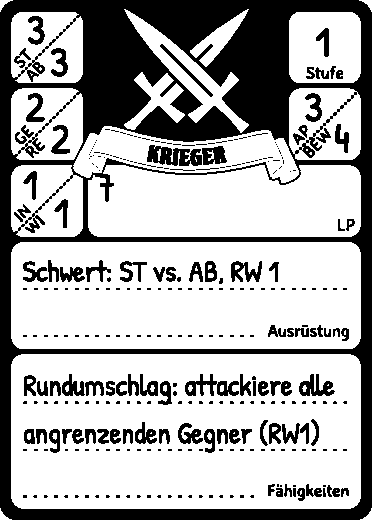
\includegraphics[angle=1,width=1\columnwidth]{\image{bmh/charsheet-fighter.pdf}}

	\newpage

	\centering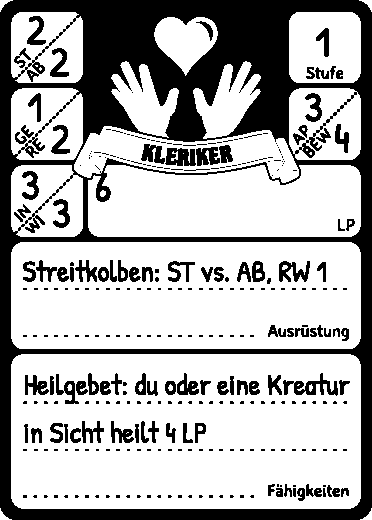
\includegraphics[angle=1.25,width=1\columnwidth]{\image{bmh/charsheet-cleric.pdf}}

	\vfill

	\centering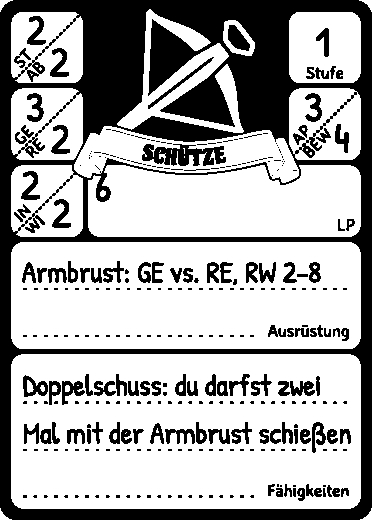
\includegraphics[angle=-1.5,width=1\columnwidth]{\image{bmh/charsheet-ranger.pdf}}

	\vfill

	\centering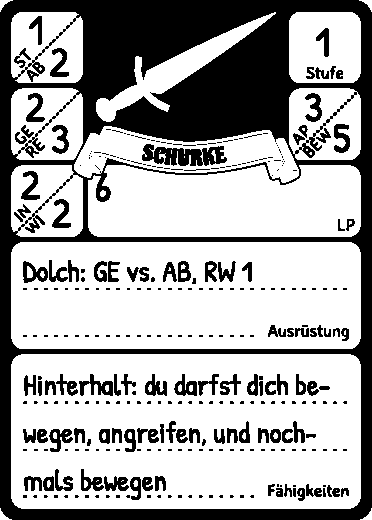
\includegraphics[angle=-1,width=1\columnwidth]{\image{bmh/charsheet-thief.pdf}}

	\vfill

	\centering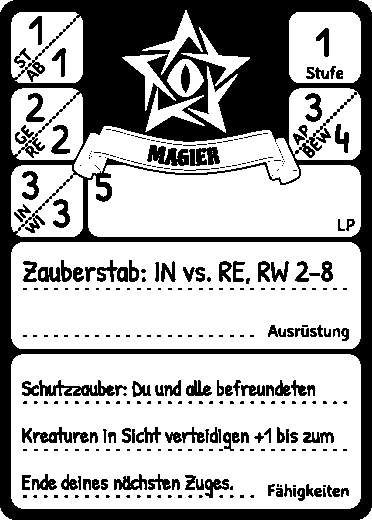
\includegraphics[angle=1.25,width=1\columnwidth]{\image{bmh/charsheet-wizard.pdf}}

}

\newcommand{\bmhMiscCharSheets}{Leere Heldenbögen}
\newcommand{\bmhMiscCharSheetsToc}{Leere Heldenbögen}

\newcommand{\bmhMiscHalt}{{%
	\vspace*{5cm}

	\centering

	{\Large \fffancy

		{\Huge HALT!}

		\bigskip

		Du kennst nun genug Regeln, um\\
		\bmh~zu spielen. \\
		Ehe du zu den Experten-Regeln \\
		übergehst, spiele erst ein paar \\
		der Missionen!\\

	}

	\vfill

}}

\newcommand{\bmhMiscMissionsHeadline}{Missionen}
\newcommand{\bmhMiscMissionsToc}{Missionen}
\newcommand{\bmhMiscMissions}{%
	MISSIONEN

	\bigskip

	\huge
	Die folgenden Seiten sind nur\\
	für den Spielleiter bestimmt.
}

\newcommand{\bmhMiscAppendixHeadline}{ANHANG}
\newcommand{\bmhMiscAppendixToc}{Anhang}
\newcommand{\bmhMiscIndexHeadline}{Index}
\newcommand{\bmhMiscIndexToc}{Index}
\newcommand{\bmhMiscBackcover}{%
	\bmh~ist eine Mischung aus Brett- und Rollenspiel für 2--5 Spieler ab 10 Jahren. In einer Fantasy-Welt voller Abenteuer, Magie und Gefahren werdet ihr als Kämpfer, Magier, Kleriker oder Schurke in alte Gemäuer hinabsteigen, sie Feld für Feld erkunden, Monster bekämpfen, Geheimnisse lüften und Schätze bergen.

	\bigskip

	Nur als Gruppe könnt ihr die Bedrohungen meistern, die den Kräften eines Einzelnen überlegen sind. Jede Mission konfrontiert euch mit neuen Herausforderungen, die sich langsam auf dem Spielplan vor euch entfalten.

}
